\paragraph{QuizziPedia::Front-End::Directives::QuestionnaireDetailsDirective}

\label{QuizziPedia::Front-End::Directives::QuestionnaireDetailsDirective}

\begin{figure}[ht]
	\centering
	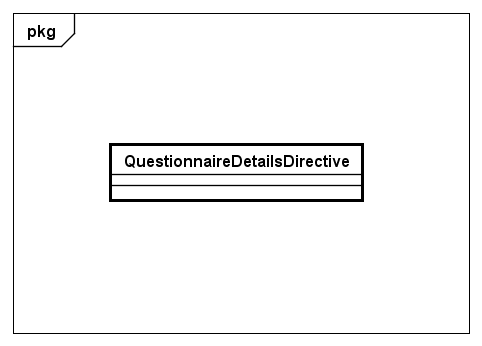
\includegraphics[scale=0.80,keepaspectratio]{UML/Classi/Front-End/QuizziPedia_Front-end_Directives_QuestionnaireDetailsDirective.png}
	\caption{QuizziPedia::Front-End::Directives::QuestionnaireDetailsDirective}
\end{figure} 
\FloatBarrier

\begin{itemize}
	\item \textbf{Descrizione}: rappresenta il componente grafico che permette all'utente di visualizzare la lista di questionari che può compilare. Ogni elemento di questa lista contiene:
		\begin{itemize}
			\item Nome del questionario;
			\item Autore del questionario;
			\item Argomento del questionario;
			\item Parole chiave del questionario.
		\end{itemize}
	Al verificarsi dell'evento click su un elemento della lista l'utente verrà indirizzato alla \textit{view\ped{G}} per la compilazione del questionario selezionato;
	\item \textbf{Utilizzo}: viene utilizzato per permettere all'utente di visualizzare la lista di questionari che può compilare;
	\item \textbf{Relazioni con altre classi}: 
	\begin{itemize}
		\item \textbf{IN \texttt{UserView}}: \textit{view\ped{G}} contenente i dati personali dell'utente, le sue statistiche relative ai questionari e agli allenamenti effettuati e i questionari a cui è iscritto;
		\item \textbf{IN \texttt{QuestionnaireDetailsController}}: questa classe permette di gestire i dettagli di un questionario;
		\item \textbf{IN \texttt{QuestionnaireDetailsModelView}}: classe di tipo \textit{modelview\ped{G}} la cui istanziazione è contenuta all'interno della variabile di ambiente \$scope di \textit{Angular\ped{G}}. All'interno di essa sono presenti le variabili e i metodi necessari per il \textit{Two-Way Data-Binding\ped{G}} tra la \textit{view\ped{G}} \texttt{UserView} e il \textit{controller\ped{G}} \texttt{QuestionnaireDetailsController};
		\item \textbf{IN \texttt{LangModel}}: rappresenta il modello delle informazioni per la giusta traduzione dell'applicazione. 
	\end{itemize}
	\item \textbf{Attributi}: 
	\begin{itemize}
		\item \texttt{+ questionnaireDetails: Object} \\ Oggetto contenente i seguenti campi dati:
		\begin{itemize}
			\item \texttt{name: String}\\ Nome del questionario;
			\item \texttt{author: String}\\ Autore del questionario;
			\item \texttt{topic: String}\\ Argomento del questionario;
			\item \texttt{keywords: Array<String>}\\ Parole chiave del questionario.
		\end{itemize}
		\item \texttt{+ compileButton: String} \\ Attributo che viene utilizzato per visualizzare la giusta traduzione della \textit{label\ped{G}} per il bottone di compilazione del questionario, in italiano o in inglese;
		\item \texttt{+ controller: String} \\ Stringa contenente il nome del \textit{controller\ped{G}} della direttiva;
		\item \texttt{+ restrict: String} \\ Stringa che permette di definire le modalità di inserimento della direttiva all'interno della pagina;
		\item \texttt{+ scope: Scope} \\ Oggetto scope interno della direttiva, contiene le funzionalità per gestire i dati presenti all'interno;
		\item \texttt{+ templateUrl: String} \\ Stringa contenente il percorso del file \textit{HTML\ped{G}} che contiene la direttive.
	\end{itemize}
\end{itemize}